
\pdfminorversion=4 % for acroread
%\documentclass[aspectratio=169,t,xcolor={usenames,dvipsnames}]{beamer}
\documentclass[aspectratio=169,t,handout,xcolor={usenames,dvipsnames}]{beamer}
\usepackage{../beamerstyle}
\usepackage{dsfont}
\usepackage{bm}
\usepackage[english]{babel}
\usepackage[utf8]{inputenc}
\usepackage{graphicx}
\usepackage{algorithm}
\usepackage[ruled,vlined,algo2e,linesnumbered]{algorithm2e}
%\usepackage[boxed,vlined]{algorithm2e}
\usepackage{hyperref}
\usepackage{booktabs}
\usepackage{mathtools}

\usepackage{amsmath,amssymb}
\usepackage{listings}
\lstset{frame=lines,framesep=3pt,numbers=left,numberblanklines=false,basicstyle=\ttfamily\small}

\usepackage{subfig}
\usepackage{multicol}
%\usepackage{appendixnumberbeamer}
%
\usepackage{tcolorbox}

\usepackage{pgfplots}
\usepackage{tikz}
\usetikzlibrary{trees} 
\usetikzlibrary{shapes.geometric}
\usetikzlibrary{positioning,shapes,shadows,arrows,calc,mindmap}
\usetikzlibrary{positioning,fadings,through}
\usetikzlibrary{decorations.pathreplacing}
\usetikzlibrary{intersections}
\usetikzlibrary{positioning,fit,calc,shadows,backgrounds}
\pgfdeclarelayer{background}
\pgfdeclarelayer{foreground}
\pgfsetlayers{background,main,foreground}
\tikzstyle{activity}=[rectangle, draw=black, rounded corners, text centered, text width=8em]
\tikzstyle{data}=[rectangle, draw=black, text centered, text width=8em]
\tikzstyle{myarrow}=[->, thick, draw=black]

% Define the layers to draw the diagram
\pgfdeclarelayer{background}
\pgfdeclarelayer{foreground}
\pgfsetlayers{background,main,foreground}

%\usepackage{listings}
%\lstset{numbers=left,
%  showstringspaces=false,
%  frame={tb},
%  captionpos=b,
%  lineskip=0pt,
%  basicstyle=\ttfamily,
%%  extendedchars=true,
%  stepnumber=1,
%  numberstyle=\small,
%  xleftmargin=1em,
%  breaklines
%}

 
\definecolor{blue}{RGB}{0, 74, 153}

\usetheme{Boadilla}
%\useinnertheme{rectangles}
\usecolortheme{whale}
\setbeamercolor{alerted text}{fg=blue}
\useoutertheme{infolines}
\setbeamertemplate{navigation symbols}{\vspace{-5pt}} % to lower the logo
\setbeamercolor{date in head/foot}{bg=white} % blue
\setbeamercolor{date in head/foot}{fg=white}
\setbeamercolor{author  in head/foot}{bg=white} %blue
\setbeamercolor{title in head/foot}{bg=white} % blue
\setbeamercolor{title}{fg=white, bg=blue}
\setbeamercolor{block title}{fg=white,bg=blue}
\setbeamercolor{block body}{bg=blue!10}
\setbeamercolor{frametitle}{fg=white, bg=blue}
\setbeamercovered{invisible}

\makeatletter
\setbeamertemplate{footline}
{
  \leavevmode%
  \hbox{%
  \begin{beamercolorbox}[wd=.333333\paperwidth,ht=2.25ex,dp=1ex,center]{author in head/foot}%
%    \usebeamerfont{author in head/foot}\insertshortauthor
  \end{beamercolorbox}%
  \begin{beamercolorbox}[wd=.333333\paperwidth,ht=2.25ex,dp=1ex,center]{title in head/foot}%
    \usebeamerfont{title in head/foot}\insertshorttitle
  \end{beamercolorbox}%
  \begin{beamercolorbox}[wd=.333333\paperwidth,ht=2.25ex,dp=1ex,right]{date in head/foot}%
    \usebeamerfont{date in head/foot}\insertshortdate{}\hspace*{2em}
%    \insertframenumber\hspace*{2ex} 
  \end{beamercolorbox}}%
  \vskip0pt%
}
\makeatother

%\pgfdeclareimage[height=1.2cm]{automl}{images/logos/automl.png}
%\pgfdeclareimage[height=1.2cm]{freiburg}{images/logos/freiburg}

%\logo{\pgfuseimage{freiburg}}

\renewcommand{\comment}[1]{
	\noindent
	%\vspace{0.25cm}
	{\color{red}{\textbf{TODO:} #1}}
	%\vspace{0.25cm}
}
\newcommand{\notefh}[1]{\textcolor{red}{\textbf{FH:} #1}}
\renewcommand{\comment}[1]{}
\newcommand{\hide}[1]{}
\newcommand{\cemph}[2]{\emph{\textcolor{#1}{#2}}}

\newcommand{\lit}[1]{{\footnotesize\color{black!60}[#1]}}

\newcommand{\litw}[1]{{\footnotesize\color{blue!20}[#1]}}


\newcommand{\myframe}[2]{\begin{frame}[c]{#1}#2\end{frame}}
\newcommand{\myframetop}[2]{\begin{frame}{#1}#2\end{frame}}
\newcommand{\myit}[1]{\begin{itemize}#1\end{itemize}}
\newcommand{\myblock}[2]{\begin{block}{#1}#2\end{block}}


\newcommand{\votepurple}[1]{\textcolor{Purple}{$\bigstar$}}
\newcommand{\voteyellow}[1]{\textcolor{Goldenrod}{$\bigstar$}}
\newcommand{\voteblue}[1]{\textcolor{RoyalBlue}{$\bigstar$}}
\newcommand{\votepink}[1]{\textcolor{Pink}{$\bigstar$}}

\newcommand{\diff}{\mathop{}\!\mathrm{d}}
\newcommand{\refstyle}[1]{{\small{\textcolor{gray}{#1}}}}
\newcommand{\hands}[0]{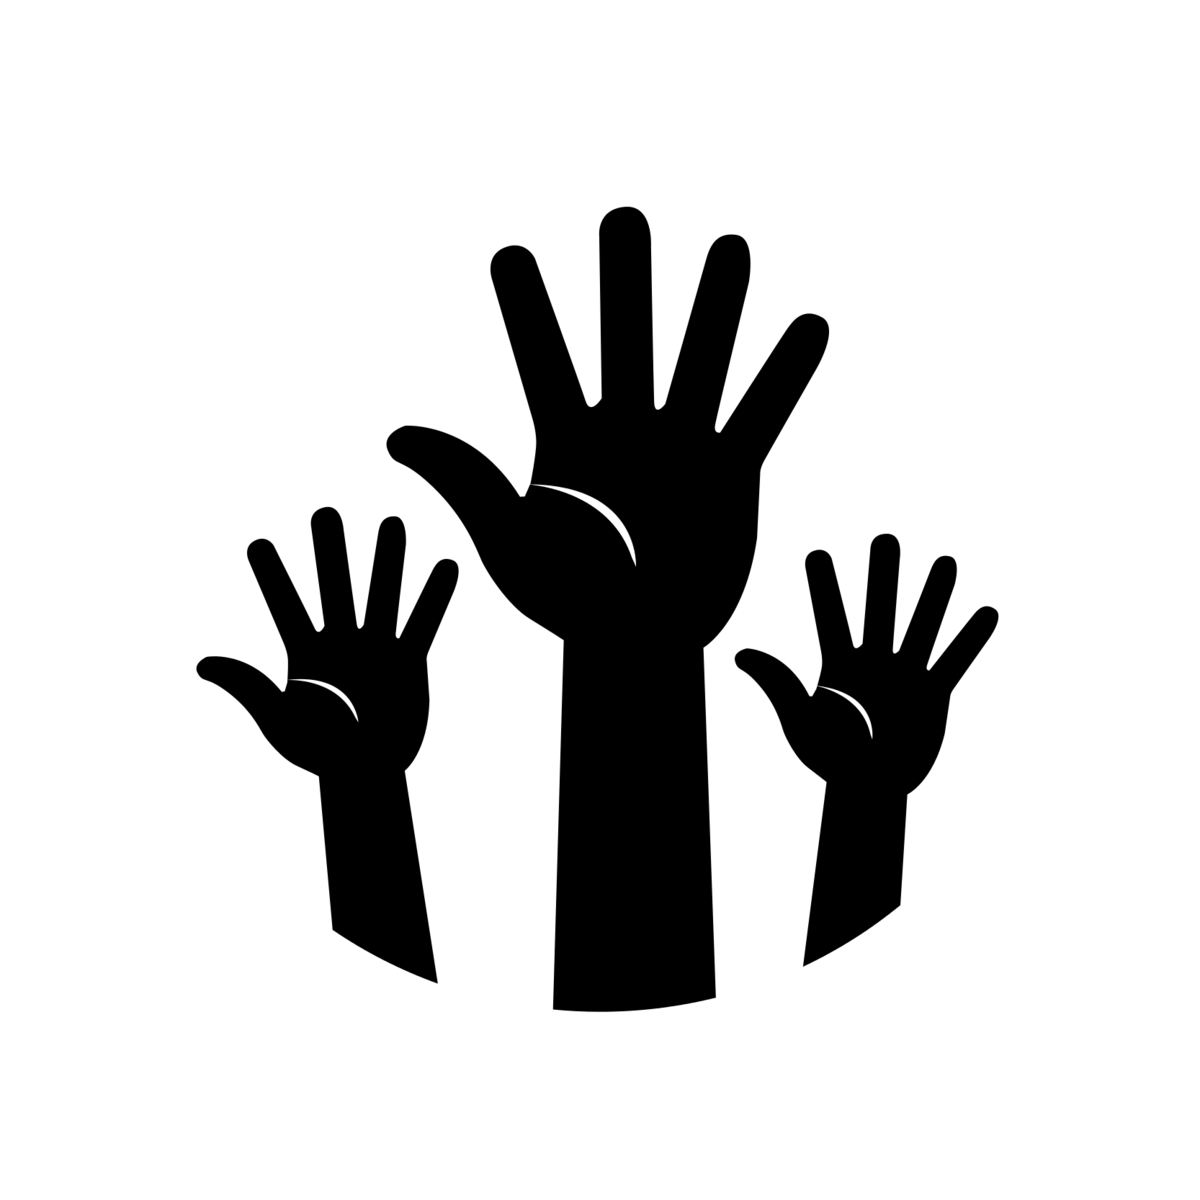
\includegraphics[height=1.5em]{images/hands}}
\newcommand{\transpose}[0]{{\textrm{\tiny{\sf{T}}}}}
\newcommand{\norm}{{\mathcal{N}}}
\newcommand{\cutoff}[0]{\kappa}
\newcommand{\instD}[0]{\dataset}
\newcommand{\insts}[0]{\mathcal{I}}
\newcommand{\inst}[0]{i}
\newcommand{\instI}[1]{i^{(#1)}}

% Iteration specific instance of variable/function/anything
% Introduced in the BO section, but moved up here to make it available within other macros
\newcommand{\iter}[2][\bocount]{{#2}^{(#1)}}

%--------HPO parameter macros-----------

% Parameter Configuration Space
\newcommand{\pcs}[0]{\pmb{\Lambda}}

% ???
\newcommand{\bx}[0]{\conf}

% Parameter Configuration
\newcommand{\conf}[0]{\pmb{\lambda}}

% Final Configuration
\newcommand{\finconf}[0]{\pmb{\hat{\lambda}}}

% Configuration corresponding to a given iteration -- better use \iter!
\newcommand{\confI}[1]{{\conf}^{(#1)}}

% Default Configuration
\newcommand{\defconf}[0]{{\conf}_{\text{def}}}

% Incumbent Configuration
\newcommand{\incumbent}[1][\bocount]{\iter[#1]{\finconf}}

% Optimal Configuration
\newcommand{\optconf}[0]{{\conf}^*}

% Configuration Space
\newcommand{\confs}[0]{\pcs}

%----------------------------------------

%\newcommand{\vlambda}[0]{\bm{\lambda}}
%\newcommand{\vLambda}[0]{\bm{\Lambda}}
\newcommand{\dataset}[0]{\mathcal{D}}
\newcommand{\datasets}[0]{\mathbf{D}}
\newcommand{\loss}[0]{L}
\newcommand{\risk}{\mathcal{R}}
\newcommand{\riske}{\mathcal{R}_{\text{emp}}}
\newcommand{\cost}[0]{c}
\newcommand{\costI}[1]{c^{(#1)}}

% Gaussian Process
\newcommand{\gp}{\mathcal{G}}
% Family of Objective Functions
\newcommand{\objF}{F}

%---------------BO Macros------------------

% BO loop counter
\newcommand{\bocount}{t}
% BO loop counter max, the counter runs from 1 to this value
\newcommand{\bobudget}{T}
% BO loop observation
\newcommand{\obs}[1][\conf]{\cost({#1})}
% BO loop observation space
\newcommand{\obsspace}{\mathcal{Y}}
% BO loop next observation
\newcommand{\bonextobs}{\obs[\iter{\conf}]}
% Acquisition Function, no args
\newcommand{\acq}{u}
% Standard Normal PDF
\newcommand{\pdf}{\phi}
% Standard Normal CDF
\newcommand{\cdf}{\Phi}
% Mean
\newcommand{\mean}{\mu}
% Standard Deviation
\newcommand{\stddev}{\sigma}
% Variance
\newcommand{\variance}{\sigma^2}
% Noise
\newcommand{\noise}{\nu}
% BO loop next selected sample
\newcommand{\bonextsample}{\confI{\bocount}}

% Single hyperparameter
\newcommand{\hyperparam}{\lambda}

% Single hyperparameter within a hyperparameter configuration
\newcommand{\hyperparami}[1][i]{{\hyperparam}_#1}

% Full definition of final configuration
\newcommand{\finconffull}{\incumbent[\bobudget]}

% Dataset
\newcommand{\datasetHPO}{{\dataset}_{HPO}}

% Dataset definition
\newcommand{\datasetHPOdef}{{\langle \bonextsample,\,\bonextobs \rangle}_{\bocount=1}^{\bobudget}}

% Double Display Fraction, forces large displays for everything in numerator and denominator
\newcommand\ddfrac[2]{\frac{\displaystyle #1}{\displaystyle #2}}

% Conditional Probability "Given That" Relation, source:https://tex.stackexchange.com/a/141685/205886
\newcommand\given[1][]{\:#1\vert\:}

% Expectation as a math operator
\DeclareMathOperator*{\E}{\mathbb{E}}

% Citation 
\newcommand{\source}[1]{
    \begin{flushright}
    	Source: \lit{#1}
    \end{flushright}
}
%-------------------------------------------

%Real numbers set
\newcommand{\realnum}{\mathbb{R}}
%Configuration space - do not use
%\newcommand{\configspace}{\Theta}
%Instances - do not use
%\newcommand{\instances}{\mathcal{I}}
%Expected value
\newcommand{\expectation}{\mathbb{E}}
%Kernel
\newcommand{\kernel}{\kappa}
%Constraint function
\newcommand{\constraintf}{c}
%Normal distribution
\newcommand{\normaldist}{\mathcal{N}}

% \renewcommand{\vec}[1]{\mathbf{#1}}
\newcommand{\hist}[0]{\dataset_{\text{Hist}}}
\newcommand{\param}[0]{p}
\newcommand{\algo}[0]{\mathcal{A}}
\newcommand{\algos}[0]{\mathbf{A}}
%\newcommand{\nn}[0]{N}
\newcommand{\feats}[0]{\mathcal{X}_{\text{meta}}}
\newcommand{\feat}[0]{\x_{\text{meta}}}
%\newcommand{\cluster}[0]{\vec{h}}
%\newcommand{\clusters}[0]{\vec{H}}
\newcommand{\perf}[0]{\mathbb{R}}
%\newcommand{\surro}[0]{\mathcal{S}}
\newcommand{\surro}[0]{\hat{\cost}}
\newcommand{\func}[0]{f}
\newcommand{\epm}[0]{\surro}
\newcommand{\portfolio}[0]{\mathbf{P}}
\newcommand{\schedule}[0]{\mathcal{S}}

% Machine Learning
\newcommand{\mdata}[0]{\dataset_{\text{meta}}}
\newcommand{\datasettrain}[0]{\dataset_{\text{train}}}
\newcommand{\datasetval}[0]{\dataset_{\text{val}}}
\newcommand{\datasettest}[0]{\dataset_{\text{test}}}
\newcommand{\x}[0]{\mathbf{x}}
\newcommand{\y}[0]{y}
\newcommand{\xI}[1]{\mathbf{x}^{(#1)}}
\newcommand{\yI}[1]{y^{(#1)}}
\newcommand{\fx}{f(\mathbf{x})}  % f(x), continuous prediction function
\newcommand{\Hspace}{\mathcal{H}} % hypothesis space where f is from
\newcommand{\fh}{\hat{f}}       % f hat, estimated prediction function

% Deep Learning
\newcommand{\weights}[0]{\theta}
\newcommand{\metaweights}[0]{\phi}


% reinforcement learning
\newcommand{\policies}[0]{\mathbf{\Pi}}
\newcommand{\policy}[0]{\pi}
\newcommand{\actionRL}[0]{a}
\newcommand{\stateRL}[0]{s}
\newcommand{\statesRL}[0]{\mathcal{S}}
\newcommand{\rewardRL}[0]{r}
\newcommand{\rewardfuncRL}[0]{\mathcal{R}}

\RestyleAlgo{algoruled}
\DontPrintSemicolon
\LinesNumbered
\SetAlgoVlined
\SetFuncSty{textsc}

\SetKwInOut{Input}{Input}
\SetKwInOut{Output}{Output}
\SetKw{Return}{return}

%\newcommand{\changed}[1]{{\color{red}#1}}

%\newcommand{\citeN}[1]{\citeauthor{#1}~(\citeyear{#1})}

\renewcommand{\vec}[1]{\mathbf{#1}}
\DeclareMathOperator*{\argmin}{arg\,min}
\DeclareMathOperator*{\argmax}{arg\,max}

%\newcommand{\aqme}{\textit{AQME}}
%\newcommand{\aslib}{\textit{ASlib}}
%\newcommand{\llama}{\textit{LLAMA}}
%\newcommand{\satzilla}{\textit{SATzilla}}
%\newcommand{\satzillaY}[1]{\textit{SATzilla'{#1}}}
%\newcommand{\snnap}{\textit{SNNAP}}
%\newcommand{\claspfolioTwo}{\textit{claspfolio~2}}
%\newcommand{\flexfolio}{\textit{FlexFolio}}
%\newcommand{\claspfolioOne}{\textit{claspfolio~1}}
%\newcommand{\isac}{\textit{ISAC}}
%\newcommand{\eisac}{\textit{EISAC}}
%\newcommand{\sss}{\textit{3S}}
%\newcommand{\sunny}{\textit{Sunny}}
%\newcommand{\ssspar}{\textit{3Spar}}
%\newcommand{\cshc}{\textit{CSHC}}
%\newcommand{\cshcpar}{\textit{CSHCpar}}
%\newcommand{\measp}{\textit{ME-ASP}}
%\newcommand{\aspeed}{\textit{aspeed}}
%\newcommand{\autofolio}{\textit{AutoFolio}}
%\newcommand{\cedalion}{\textit{Cedalion}}
\newcommand{\fanova}{\textit{fANOVA}}
\newcommand{\sbs}{\textit{SB}}
\newcommand{\oracle}{\textit{VBS}}

% like approaches
\newcommand{\claspfoliolike}[1]{\texttt{claspfolio-#1-like}}
\newcommand{\satzillalike}[1]{\texttt{SATzilla'#1-like}}
\newcommand{\isaclike}{\texttt{ISAC-like}}
\newcommand{\ssslike}{\texttt{3S-like}}
\newcommand{\measplike}{\texttt{ME-ASP-like}}

\newcommand{\irace}{\textit{I/F-race}}
\newcommand{\gga}{\textit{GGA}}
\newcommand{\smac}{\textit{SMAC}}
\newcommand{\paramils}{\textit{ParamILS}}
\newcommand{\spearmint}{\textit{Spearmint}}
\newcommand{\tpe}{\textit{TPE}}


\usepackage{pifont}
\newcommand{\itarrow}{\mbox{\Pisymbol{pzd}{229}}}
\newcommand{\ithook}{\mbox{\Pisymbol{pzd}{52}}}
\newcommand{\itcross}{\mbox{\Pisymbol{pzd}{56}}}
\newcommand{\ithand}{\mbox{\raisebox{-1pt}{\Pisymbol{pzd}{43}}}}

%\DeclareMathOperator*{\argmax}{arg\,max}

\newcommand{\ie}{{\it{}i.e.\/}}
\newcommand{\eg}{{\it{}e.g.\/}}
\newcommand{\cf}{{\it{}cf.\/}}
\newcommand{\wrt}{\mbox{w.r.t.}}
\newcommand{\vs}{{\it{}vs\/}}
\newcommand{\vsp}{{\it{}vs\/}}
\newcommand{\etc}{{\copyedit{etc.}}}
\newcommand{\etal}{{\it{}et al.\/}}

\newcommand{\pscProc}{{\bf procedure}}
\newcommand{\pscBegin}{{\bf begin}}
\newcommand{\pscEnd}{{\bf end}}
\newcommand{\pscEndIf}{{\bf endif}}
\newcommand{\pscFor}{{\bf for}}
\newcommand{\pscEach}{{\bf each}}
\newcommand{\pscThen}{{\bf then}}
\newcommand{\pscElse}{{\bf else}}
\newcommand{\pscWhile}{{\bf while}}
\newcommand{\pscIf}{{\bf if}}
\newcommand{\pscRepeat}{{\bf repeat}}
\newcommand{\pscUntil}{{\bf until}}
\newcommand{\pscWithProb}{{\bf with probability}}
\newcommand{\pscOtherwise}{{\bf otherwise}}
\newcommand{\pscDo}{{\bf do}}
\newcommand{\pscTo}{{\bf to}}
\newcommand{\pscOr}{{\bf or}}
\newcommand{\pscAnd}{{\bf and}}
\newcommand{\pscNot}{{\bf not}}
\newcommand{\pscFalse}{{\bf false}}
\newcommand{\pscEachElOf}{{\bf each element of}}
\newcommand{\pscReturn}{{\bf return}}

%\newcommand{\param}[1]{{\sl{}#1}}
\newcommand{\var}[1]{{\it{}#1}}
\newcommand{\cond}[1]{{\sf{}#1}}
%\newcommand{\state}[1]{{\sf{}#1}}
%\newcommand{\func}[1]{{\sl{}#1}}
\newcommand{\set}[1]{{\Bbb #1}}
%\newcommand{\inst}[1]{{\tt{}#1}}
\newcommand{\myurl}[1]{{\small\sf #1}}

\newcommand{\Nats}{{\Bbb N}}
\newcommand{\Reals}{{\Bbb R}}
\newcommand{\extset}[2]{\{#1 \; | \; #2\}}

\newcommand{\vbar}{$\,\;|$\hspace*{-1em}\raisebox{-0.3mm}{$\,\;\;|$}}
\newcommand{\vendbar}{\raisebox{+0.4mm}{$\,\;|$}}
\newcommand{\vend}{$\,\:\lfloor$}


\newcommand{\goleft}[2][.7]{\parbox[t]{#1\linewidth}{\strut\raggedright #2\strut}}
\newcommand{\rightimage}[2][.3]{\mbox{}\hfill\raisebox{1em-\height}[0pt][0pt]{\includegraphics[width=#1\linewidth]{#2}}\vspace*{-\baselineskip}}






\newcommand{\lz}{\vspace{0.5cm}}
\newcommand{\thetab}{\bm{\weights}}
\newcommand{\zero}{\mathbf{0}}
\newcommand{\Xmat}{\mathbf{X}}
\newcommand{\ydat}{\mathbf{y}}
\newcommand{\id}{\boldsymbol{I}}
\newcommand{\Amat}{\mathbf{A}}
\newcommand{\Xspace}{\mathcal{X}}                                           
\newcommand{\Yspace}{\mathcal{Y}}
\newcommand{\ls}{\ell}
\newcommand{\natnum}{\mathbb{N}}
\newcommand{\intnum}{\mathbb{Z}}
\newcommand{\Kmat}{\bm{K}}


\usepackage{fontawesome}
\usepackage{dirtytalk}
\usepackage{csquotes}

\def\argmin{\mathop{\sf arg\,min}}   

%\begin{frame}[c]{}
%\centering
%\huge
%\textbf{}
%\end{frame}


%\item[\faLightbulbO]

%\(\xI{i},\yI{i})


\title[AutoML: GPs]{AutoML: Gaussian Processes} % week title
\subtitle{Gaussian Process Prediction} % video title
\author[Marius Lindauer]{\underline{Bernd Bischl} \and Frank Hutter \and Lars Kotthoff\newline \and Marius Lindauer \and Joaquin Vanschoren}
\institute{}
\date{}




\begin{document}
\maketitle



%%%%%%%%%%%%%%%%%%%%%%%%%%%%%%%%%%%%%%%%%%%%%%%%%%%%%%%%%%%%%%%%%%%%%%%%%%%%%%%%%%%%
\begin{frame}[c]{Motivation}

\begin{itemize}

\item So far, we have learned how to \textbf{sample} from a Gaussian process prior.
\lz
\item However, most of the time, we are not interested in drawing random functions from the prior. Instead, we usually like to use the knowledge provided by the training data to predict values of $f$ at a new test point $\x_*$. 
\lz
\item In what follows, we will investigate how to update the Gaussian process prior ($\to$ posterior process) and how to make predictions.


\end{itemize}


\end{frame}
%%%%%%%%%%%%%%%%%%%%%%%%%%%%%%%%%%%%%%%%%%%%%%%%%%%%%%%%%%%%%%%%%%%%%%%%%%%%%%%%%%%%
\begin{frame}[c]{}
\centering
\huge
\textbf{Gaussian Posterior Process and Prediction}
\end{frame}


%%%%%%%%%%%%%%%%%%%%%%%%%%%%%%%%%%%%%%%%%%%%%%%%%%%%%%%%%%%%%%%%%%%%%%%%%%%%%%%%%%%%
\begin{frame}[c,allowframebreaks]{Posterior Process}

\begin{itemize}
\item Let us distinguish between \textbf{observed training} inputs (also denoted by a design matrix $\Xmat$), their corresponding values
  
$$\bm{f} = \left[f\left(\xI{1}\right),\dots, f\left(\xI{n}\right)\right],$$ 

and one single \textbf{unobserved test point} $\x_*$ with $f_* = f\left(\x_*\right).$

\item We now want to infer the distribution of $f_* | x_*, X, \bm{f}$.

\item Assuming a zero-mean GP prior $\gp\left(\bm{0}, k(\x, \x^\prime)\right)$, we can assert that
$$\begin{bmatrix}\bm{f} \\
f_*\end{bmatrix}\sim  
\normaldist\biggl(\bm{0}, \begin{bmatrix} \bm{K} & \bm{k}_* \\ \bm{k}_*^T & \bm{k}_{**}\end{bmatrix}\biggr),$$

where, $\bm{K} = \left(k\left(\xI{i}, \xI{j}\right)\right)_{i,j}$, $\bm{k}_* = \left[k\left(\x_*, \xI{1}\right),\dots, k\left(\x_*, \xI{n}\right)\right]$ and $ \bm{k}_{**}\ = k(\x_*, \x_*)$.

\end{itemize}
%%%%%%%%%%%%%%%%%%%%%%%%%%%%%%%%%%%%%%%%%%%%%%%%%%%%%%%%%%%%%%%%%%%%%%%%%%%%%%%%%%%%
\framebreak


\textit{${(*)}\,$A General Rule of Conditioning for Gaussian Random Variables}

\lz
\lz

If the $m$-dimensional Gaussian vector $\bm{z} \sim \normaldist(\mu, \Sigma)$ can be partitioned with $\bm{z} = \left(\bm{z}_1, \bm{z}_2\right)$ where $\bm{z}_1$ is $m_1$-dimensional and $\bm{z}_2$ is $m_2$-dimensional, and:
$$\left(\mu_1, \mu_2\right), \quad \Sigma = \begin{pmatrix} \Sigma_{11} & \Sigma_{12} \\ \Sigma_{21} & \Sigma_{22} \end{pmatrix},$$
then the conditional distribution $\bm{a}= \bm{z}_2 ~|~ \bm{z}_1$ will be a multivariate normal distribution:

$$
\normaldist\left(\mu_2 + \Sigma_{21} \Sigma_{11}^{-1}\left(\bm{a} - \mu_1\right), \Sigma_{22} - \Sigma_{21}\Sigma_{11}^{-1}\Sigma_{12} \right)
$$


%%%%%%%%%%%%%%%%%%%%%%%%%%%%%%%%%%%%%%%%%%%%%%%%%%%%%%%%%%%%%%%%%%%%%%%%%%%%%%%%%%%%
\framebreak


\begin{itemize}

\item Given that $\bm{f}$ is observed, we can exploit the general rule ${(*)}\,$ to obtain the following formula: 

\begin{eqnarray*}
f_* ~|~ \x_*, \Xmat, \bm{f} \sim \normaldist(\bm{k}_{*}^{T}\Kmat^{-1}\bm{f}, \bm{k}_{**} - \bm{k}_*^T \Kmat ^{-1}\bm{k}_*).
\end{eqnarray*}

\lz
\lz

\item As the posterior is Gaussian, the maximum a-posteriori estimate (i.e., the mode of the posterior distribution) is:

\large $$\bm{k}_{*}^{T}\Kmat^{-1}\bm{f}$$.

\end{itemize}
\end{frame}
%%%%%%%%%%%%%%%%%%%%%%%%%%%%%%%%%%%%%%%%%%%%%%%%%%%%%%%%%%%%%%%%%%%%%%%%%%%%%%%%%%%%
\begin{frame}[c,allowframebreaks]{GP Prediction: Two Points}

To visualize the above idea, assume that we have observed a single training point $\x = - 0.5$. Based on this point, we intend to make a prediction at the test point $\x_* = 0.5$.

\vspace{3mm}

\begin{itemize}
  \item Under a zero-mean $\gp$ with $k(\x, \x^\prime) = \exp(-\frac{1}{2}\|\x - \x^\prime\|^2)$, we compute the cov-matrix:
  \vspace{-3mm}
  $$\begin{bmatrix} f \\ f_* \end{bmatrix} \sim \normaldist\biggl(\bm{0}, \begin{bmatrix} 1 & 0.61 \\ 0.61 & 1\end{bmatrix}\biggr).$$ 
  \item Let us assume that we observe the point $f(\x) = 1$. We can compute the posterior distribution:
\vspace{-5mm}
  \begin{eqnarray*}
    f_* ~|~ \x_*, \x, f &\sim& \normaldist(\bm{k}_{*}^{T}\Kmat^{-1}f, k_{**} - \bm{k}_*^T \Kmat^{-1}\bm{k}_*) \\
    &\sim& \normaldist(0.61 \cdot 1 \cdot 1, 1 - 0.61 \cdot 1 \cdot 0.61) \\
    &\sim& \normaldist\left(0.61, 0.6279\right) 
  \end{eqnarray*}
  \item The MAP-estimate for $\x_*$ is $f(\x_*) = 0.61$, and the uncertainty estimate is $0.6279$.

\end{itemize}

\framebreak
%%%%%%%%%%%%%%%%%%%%%%%%%%%%%%%%%%%%%%%%%%%%%%%%%%%%%%%%%%%%%%%%%%%%%%%%%%%%%%%%%%%%


The figures show the bivariate normal density as well as the corresponding marginals. 


\begin{figure}
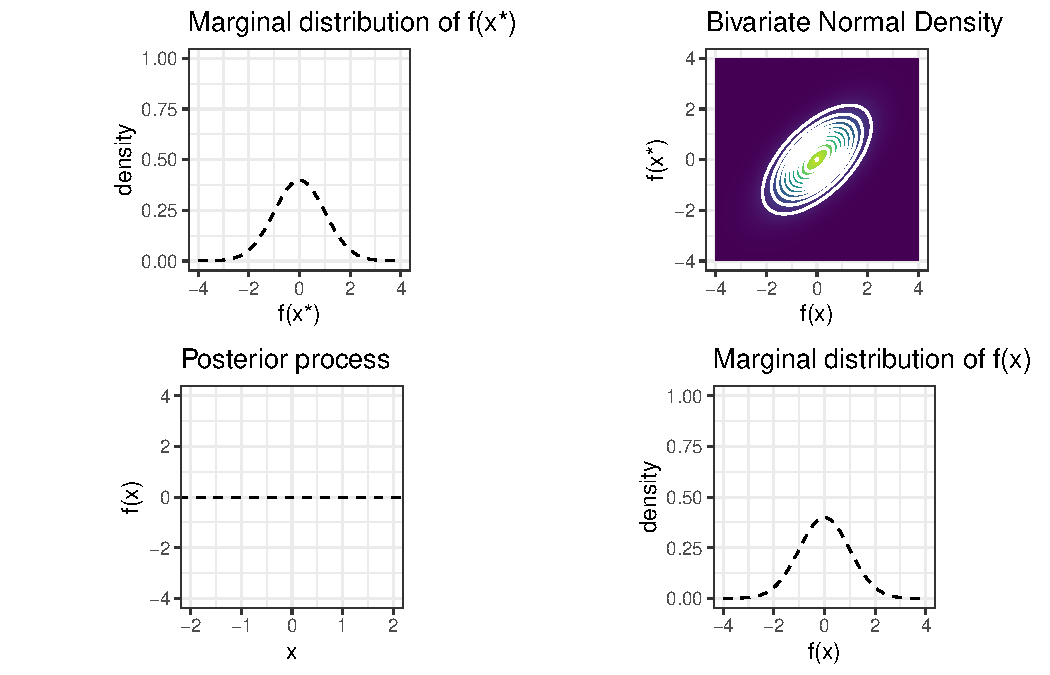
\includegraphics[width=0.6\textwidth]{figure/gp-posterior-1-1.pdf}\par
\end{figure}

\framebreak
%%%%%%%%%%%%%%%%%%%%%%%%%%%%%%%%%%%%%%%%%%%%%%%%%%%%%%%%%%%%%%%%%%%%%%%%%%%%%%%%%%%%

We observe $f(\x) = 1$ at training point $\x = -0.5$. 


\begin{figure}
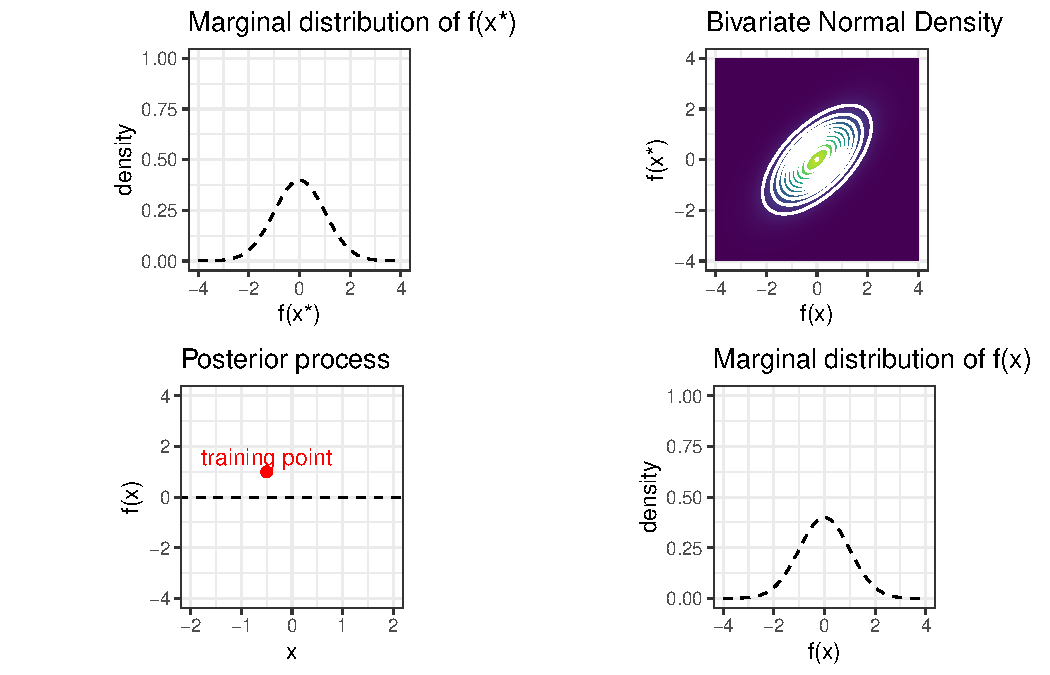
\includegraphics[width=0.6\textwidth]{figure/gp-posterior-2-1.pdf}\par
\end{figure}


\framebreak
%%%%%%%%%%%%%%%%%%%%%%%%%%%%%%%%%%%%%%%%%%%%%%%%%%%%%%%%%%%%%%%%%%%%%%%%%%%%%%%%%%%%

We condition the Gaussian on $f(\x) = 1$. 


\begin{figure}
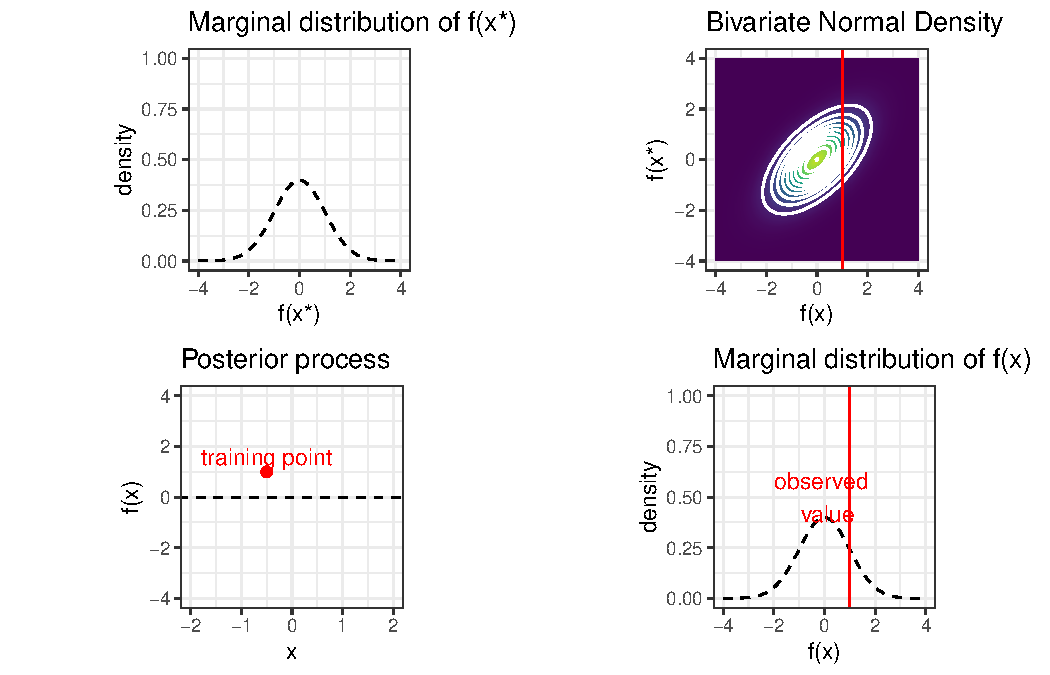
\includegraphics[width=0.6\textwidth]{figure/gp-posterior-3-1.pdf}\par
\end{figure}

\framebreak
%%%%%%%%%%%%%%%%%%%%%%%%%%%%%%%%%%%%%%%%%%%%%%%%%%%%%%%%%%%%%%%%%%%%%%%%%%%%%%%%%%%%

We then compute the posterior distribution of $f(\x_*)$ given that $\fx = 1$.


\begin{figure}
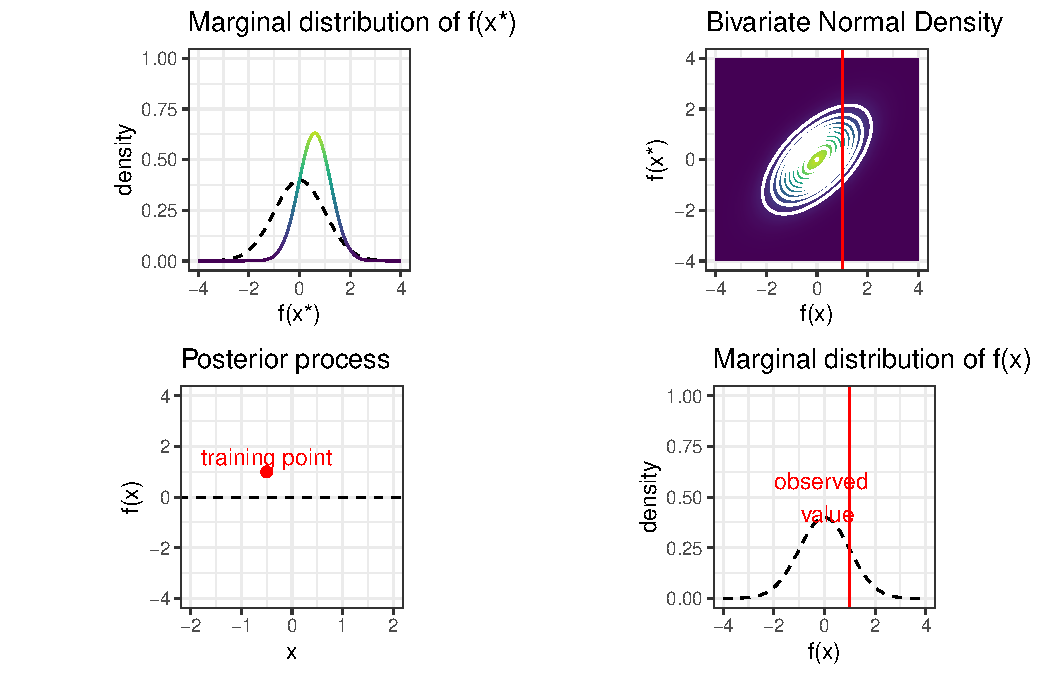
\includegraphics[width=0.6\textwidth]{figure/gp-posterior-5-1.pdf}\par
\end{figure}


\framebreak
%%%%%%%%%%%%%%%%%%%%%%%%%%%%%%%%%%%%%%%%%%%%%%%%%%%%%%%%%%%%%%%%%%%%%%%%%%%%%%%%%%%%

A possible predictor for $f$ at $\x_*$ is the MAP of the posterior distribution.


\begin{figure}
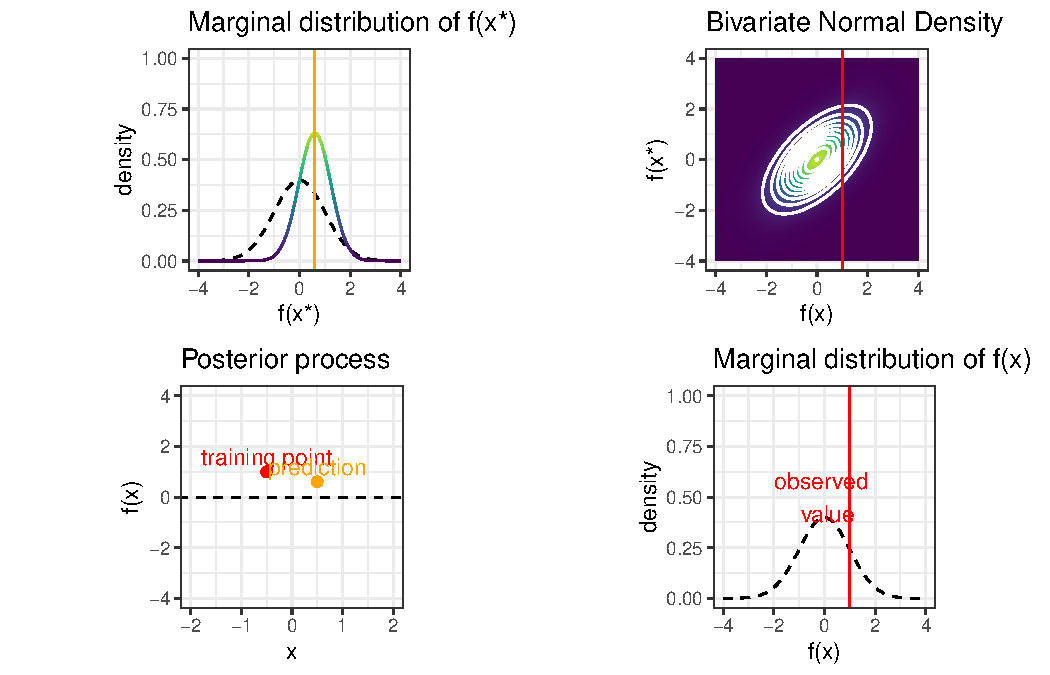
\includegraphics[width=0.6\textwidth]{figure/gp-posterior-6-1.pdf}\par
\end{figure}


\framebreak
%%%%%%%%%%%%%%%%%%%%%%%%%%%%%%%%%%%%%%%%%%%%%%%%%%%%%%%%%%%%%%%%%%%%%%%%%%%%%%%%%%%%

We can repeat this process for different $\x_*$ and find the respective mean (grey line) and standard deviation (grey area). Note that the grey area is mean $\pm 2 \times$ standard deviation.


\begin{figure}
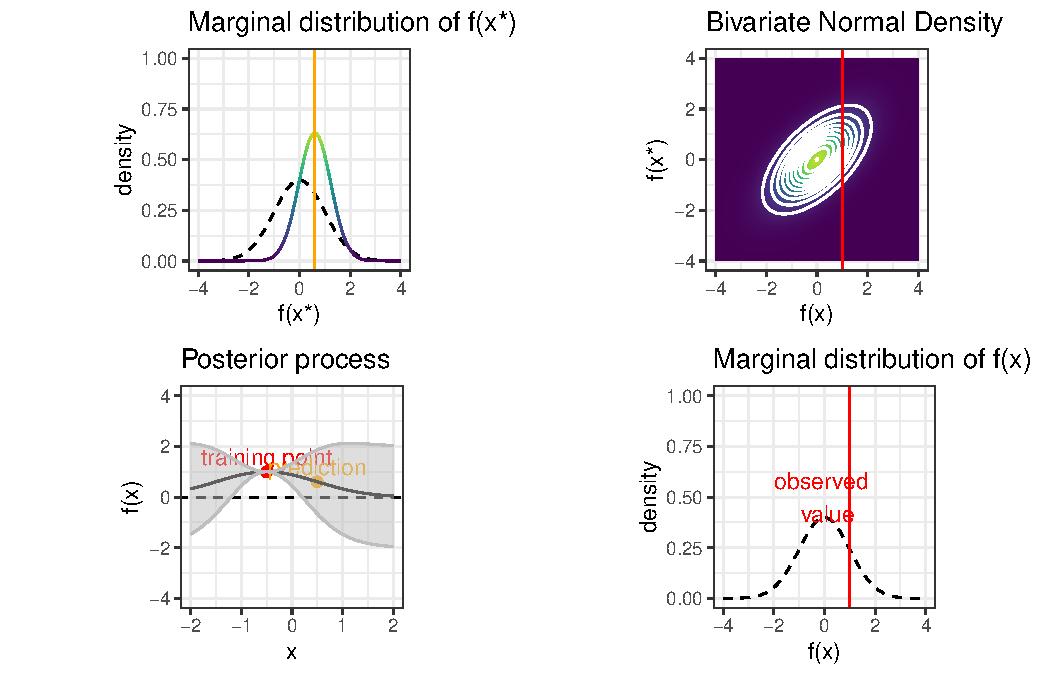
\includegraphics[width=0.55\textwidth]{figure/gp-posterior-7-1.pdf}\par
\end{figure}


\end{frame}
%%%%%%%%%%%%%%%%%%%%%%%%%%%%%%%%%%%%%%%%%%%%%%%%%%%%%%%%%%%%%%%%%%%%%%%%%%%%%%%%%%%%
\begin{frame}[c,allowframebreaks]{Posterior Process}

\begin{itemize}
\item The previous discussion was restricted to a single test point. However, one can generalize it to posterior processes with multiple unobserved test points:
  
$$\bm{f}_* = \left[f\left(\xI{1}_*\right),\dots, f\left(\xI{m}_*\right)\right].$$ 


\lz

\item Under a zero-mean Gaussian process, we have:

$$\begin{bmatrix}\bm{f} \\
\bm{f}_*\end{bmatrix}\sim  
\normaldist\biggl(\bm{0}, \begin{bmatrix} \bm{K} & \bm{K}_* \\ \bm{K}_*^T & \bm{K}_{**}\end{bmatrix}\biggr),$$

where $\bm{K}_* = \left(k\left(\xI{i}, \xI{j}_*\right)\right)_{i,j}$ and $\bm{K}_{**} = \left(k\left(\xI{i}_*, \xI{j}_*\right)\right)_{i,j}$ 

\end{itemize}

\framebreak
%%%%%%%%%%%%%%%%%%%%%%%%%%%%%%%%%%%%%%%%%%%%%%%%%%%%%%%%%%%%%%%%%%%%%%%%%%%%%%%%%%%%

\begin{itemize}

  \item Similar to the single test point situation, to get the posterior distribution, we exploit the general rule of conditioning for Gaussians:
  
  \begin{eqnarray*}
    \bm{f}_* ~|~ \Xmat_*, \Xmat, \bm{f} \sim \normaldist(\Kmat_{*}^{T}\Kmat^{-1}\bm{f}, \Kmat_{**} - \Kmat_*^T \Kmat ^{-1}\Kmat_*).
  \end{eqnarray*}  
  
\lz

  \item This formula enables us to talk about correlations among different test points and sample functions from the posterior process. 
\end{itemize}


\end{frame}

%%%%%%%%%%%%%%%%%%%%%%%%%%%%%%%%%%%%%%%%%%%%%%%%%%%%%%%%%%%%%%%%%%%%%%%%%%%%%%%%%%%%
\begin{frame}[c]{}
\centering
\huge
\textbf{Properties of a Gaussian Process}
\end{frame}
%%%%%%%%%%%%%%%%%%%%%%%%%%%%%%%%%%%%%%%%%%%%%%%%%%%%%%%%%%%%%%%%%%%%%%%%%%%%%%%%%%%%
\begin{frame}[c]{GP as an Interpolator}

\begin{itemize}

\item The  ``prediction'' for a training point $\xI{i}$ is the exact function value $f(\xI{i})$. That is, 
\begin{eqnarray*}
\bm{f} ~|~ \Xmat, \bm{f} \sim \normaldist(\Kmat\Kmat^{-1}\bm{f}, \Kmat - \Kmat^T \Kmat^{-1} \Kmat) = \normaldist(\bm{f}, \bm{0}).
\end{eqnarray*}

\item Thus, a Gaussian process is a function \textbf{interpolator}.
\end{itemize}

\begin{figure}
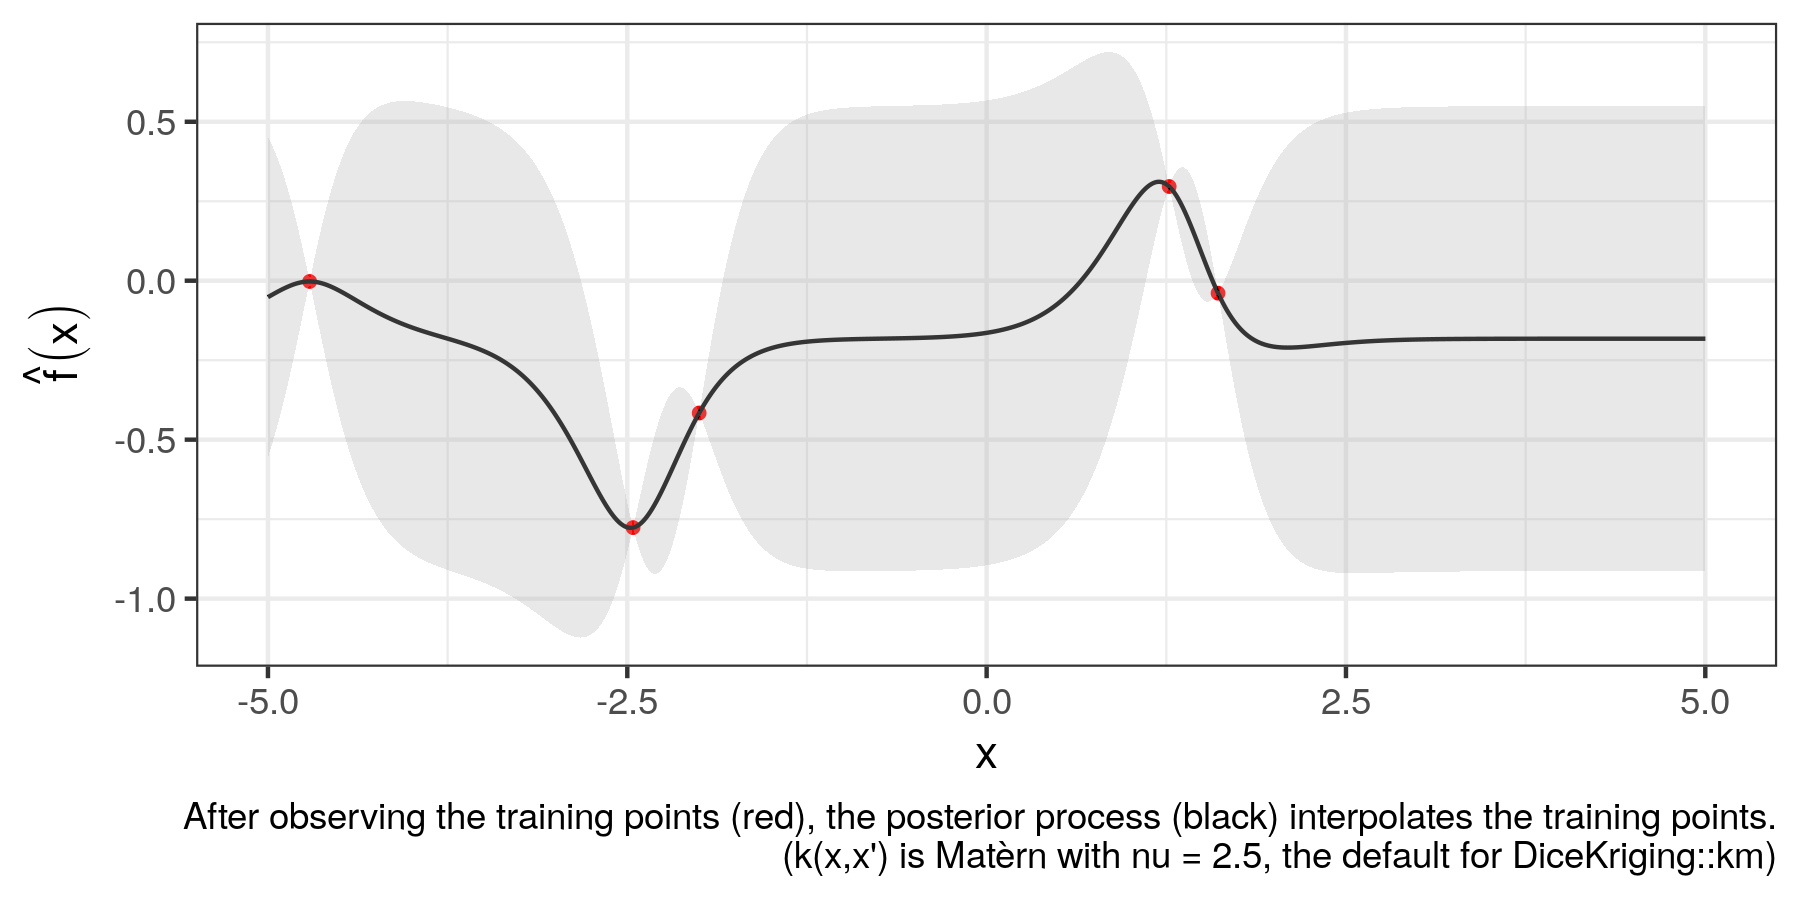
\includegraphics[width=0.6\textwidth]{figure_man/gp-interpolator.png}\par
\end{figure}

\end{frame}

%%%%%%%%%%%%%%%%%%%%%%%%%%%%%%%%%%%%%%%%%%%%%%%%%%%%%%%%%%%%%%%%%%%%%%%%%%%%%%%%%%%%
\begin{frame}[c,allowframebreaks]{GP as a Spatial Model}

\begin{itemize}
%\begin{footnotesize}
\item The correlation among two outputs depends on the distance of the coresponding input points $\x$ and $\x^\prime$. For instance, the Gaussian covariance kernel is \begin{footnotesize}$k(\x, \x^\prime) = \exp \left(\frac{- \|\x - \x^\prime\|^2}{2 \ls^2}\right)$.\end{footnotesize}
\vspace{3mm}
\item Hence, close data points with high spatial similarity $k(\x, \x^\prime)$ enter into more strongly correlated predictions: $\bm{k}_*^\top \bm{K}^{-1} \bm{f}$ ($\bm{k}_* := \left(k(\x, \xI{1}),\dots, k(\x, \xI{n})\right)$).
%\end{footnotesize}
\end{itemize}

\begin{figure}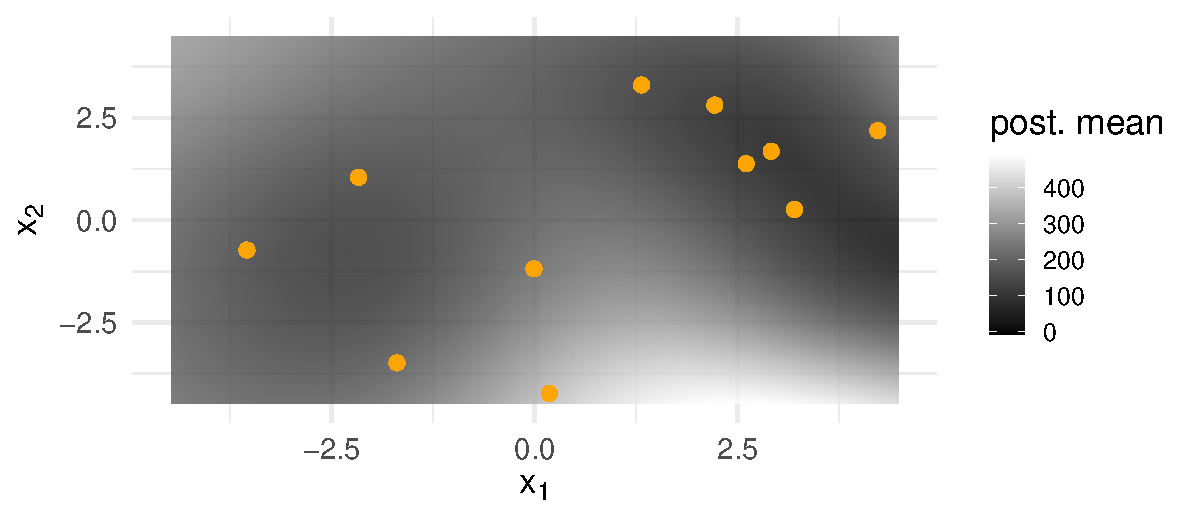
\includegraphics[width=0.62\textwidth]{figure/mbo-2d-1.pdf}\par\vspace{-3mm}\begin{footnotesize}\textbf{Example:} the posterior mean of a GP that is fitted with the Gaussian covariance kernel with $\ls = 1$.\end{footnotesize}\end{figure}

\framebreak
%%%%%%%%%%%%%%%%%%%%%%%%%%%%%%%%%%%%%%%%%%%%%%%%%%%%%%%%%%%%%%%%%%%%%%%%%%%%%%%%%%%%

\begin{itemize}

\item Posterior uncertainty increases if the new data points are far from the design points.
\lz
\item The uncertainty is minimal at the design points, since the posterior variance is zero at these points.
\end{itemize}

\begin{figure}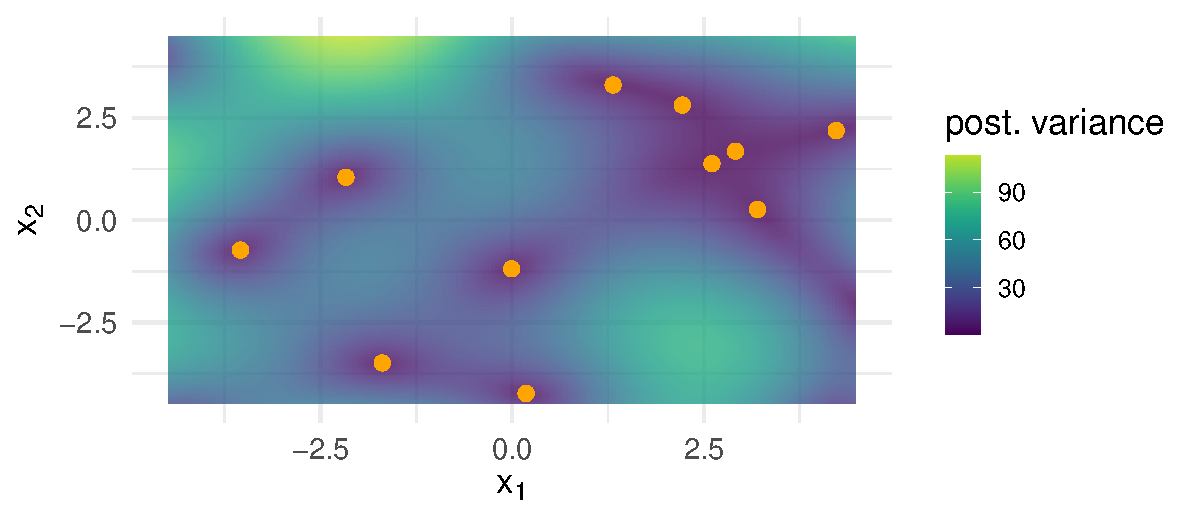
\includegraphics[width=0.68\textwidth]{figure/mbo-2d-2-1.pdf}\par
\vspace{-3mm}
\begin{footnotesize}
\textbf{Example (continued):} posterior variance
\end{footnotesize}
\end{figure}


\end{frame}
%%%%%%%%%%%%%%%%%%%%%%%%%%%%%%%%%%%%%%%%%%%%%%%%%%%%%%%%%%%%%%%%%%%%%%%%%%%%%%%%%%%%
\begin{frame}[c]{}
\centering
\huge
\textbf{Noisy Gaussian Process}
\end{frame}
%%%%%%%%%%%%%%%%%%%%%%%%%%%%%%%%%%%%%%%%%%%%%%%%%%%%%%%%%%%%%%%%%%%%%%%%%%%%%%%%%%%%
\begin{frame}[c,allowframebreaks]{Noisy Gaussian Process}

\begin{itemize}
\item So far, we have implicitely assumed that we access the true function values $f(\x)$.
\vspace{3mm}
\item For the squared exponential kernel, for example, we had
  $cov\left(f(\xI{i}), f(\xI{j})\right) = 1.$
\vspace{3mm}
\item Consequently, the posterior Gaussian process was an interpolator.
\end{itemize}

\begin{figure}
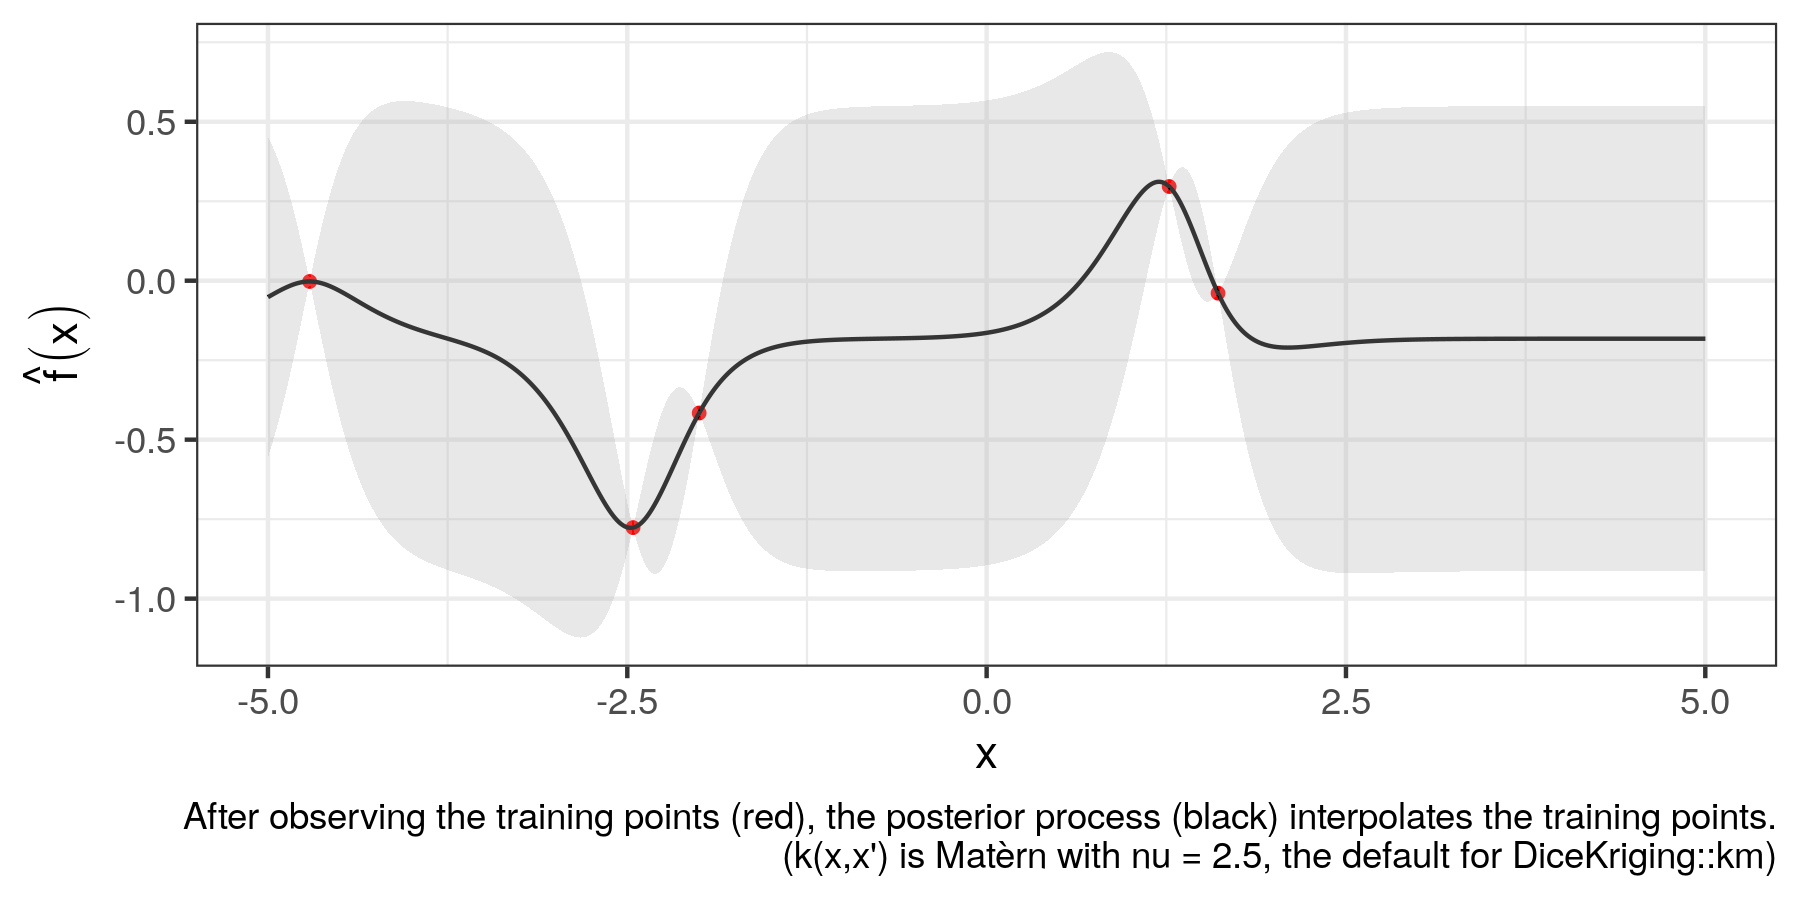
\includegraphics[width=0.6\textwidth]{figure_man/gp-interpolator.png}\par
\end{figure}

%%%%%%%%%%%%%%%%%%%%%%%%%%%%%%%%%%%%%%%%%%%%%%%%%%%%%%%%%%%%%%%%%%%%%%%%%%%%%%%%%%%%
\framebreak

\begin{itemize}

\item However, in reality that is not often the case. Rather, we often only have access to a noisy version of the true function values:
  $$y = f(\x) + \epsilon, \text{ where } \epsilon \sim\normaldist\left(0, \variance\right).$$
  
\item Let us assume that $f(\x)$ is still a Gaussian process. Then, we would have the following:
  \begin{footnotesize} 
  \begin{eqnarray*}
    &&cov\,(\yI{i}, \yI{j}) = cov\left(f\left(\xI{i}\right) + \epsilon^{(i)}, f\left(\xI{j}\right) + \epsilon^{j}\right) \\
    &=& cov\left(f\left(\xI{i}\right), f\left(\xI{j}\right)\right) + 2 \cdot cov\left(f\left(\xI{i}\right), \epsilon^{(j)}\right) + cov\left(\epsilon^{(i)}, \epsilon^{(j)}\right) 
    \\ &=& k\left(\xI{i}, \xI{j}\right) + \variance \delta_{ij}. 
  \end{eqnarray*}
  \end{footnotesize}
  \item $\variance$ is called \textbf{nugget}. 
\end{itemize}

%%%%%%%%%%%%%%%%%%%%%%%%%%%%%%%%%%%%%%%%%%%%%%%%%%%%%%%%%%%%%%%%%%%%%%%%%%%%%%%%%%%%
\framebreak

\begin{itemize}
  \item We can now derive the predictive distribution for the case of noisy observations. 
  \item Assuming that $f$ is modeled by a Gaussian process, the prior distribution of $y$ is
  
  $$\bm{y} = \begin{pmatrix} \yI{1} \\ \yI{2} \\ \vdots \\ \yI{n} \end{pmatrix} \sim \normaldist\left(\bm{m}, \bm{K} + \variance I_n \right),$$
  
  with

  \begin{eqnarray*}
    \textbf{m} &:=& \left(m\left(\xI{i}\right)\right)_{i}, \quad
    \textbf{K} := \left(k\left(\xI{i}, \xI{j}\right)\right)_{i,j}. 
  \end{eqnarray*}
\end{itemize}

\framebreak 
%%%%%%%%%%%%%%%%%%%%%%%%%%%%%%%%%%%%%%%%%%%%%%%%%%%%%%%%%%%%%%%%%%%%%%%%%%%%%%%%%%%%


We distinguish again between:

\lz

\begin{itemize}
    \item Observed training points and their corresponding values, i.e, $\Xmat$ and $\bm{y}$.
\item Unobserved test points and their corresponding values, i.e, $\Xmat_*$ and $\bm{f}_*$.
\end{itemize}

\lz

and get:
  
  $$
  \begin{bmatrix}
  \bm{y} \\
  \bm{f}_*
  \end{bmatrix} \sim  
  \normaldist\biggl(\bm{0}, \begin{bmatrix} \Kmat + \variance I_n & \Kmat_* \\ \Kmat_*^T & \Kmat_{**} \end{bmatrix}\biggr).
  $$

\framebreak
%%%%%%%%%%%%%%%%%%%%%%%%%%%%%%%%%%%%%%%%%%%%%%%%%%%%%%%%%%%%%%%%%%%%%%%%%%%%%%%%%%%%
\begin{itemize}

\item Similar to the noise-free case, we condition according to the rule of conditioning for Gaussians to get the posterior distribution for the test outputs $\bm{f}_*$ at $\Xmat_*$:

\begin{eqnarray*}
\bm{f}_* ~|~ \Xmat_*, \Xmat, \bm{y} \sim \normaldist(\bm{m}_{\text{post}}, \bm{K}_\text{post}),
\end{eqnarray*}

with 

\begin{eqnarray*}
\bm{m}_{\text{post}} &=& \Kmat_{*}^{T} \left(\Kmat+ \sigma^2 \cdot \id\right)^{-1}\bm{y} \\
\lz
\bm{K}_\text{post} &=& \Kmat_{**} - \Kmat_*^T \left(\Kmat ^{-1} + \sigma^2 \cdot \id\right)\Kmat_*.
\end{eqnarray*}

\end{itemize}

\begin{itemize}
\item This converts back to the noise-free formula if $\variance = 0$.
\end{itemize}

\framebreak
%%%%%%%%%%%%%%%%%%%%%%%%%%%%%%%%%%%%%%%%%%%%%%%%%%%%%%%%%%%%%%%%%%%%%%%%%%%%%%%%%%%%

\begin{itemize}
\item The noisy Gaussian process is not an interpolator any more.
\item A larger nugget term leads to a wider ``band'' around the observed training points.
\item The nugget term is estimated during training.
\end{itemize}


\begin{figure}
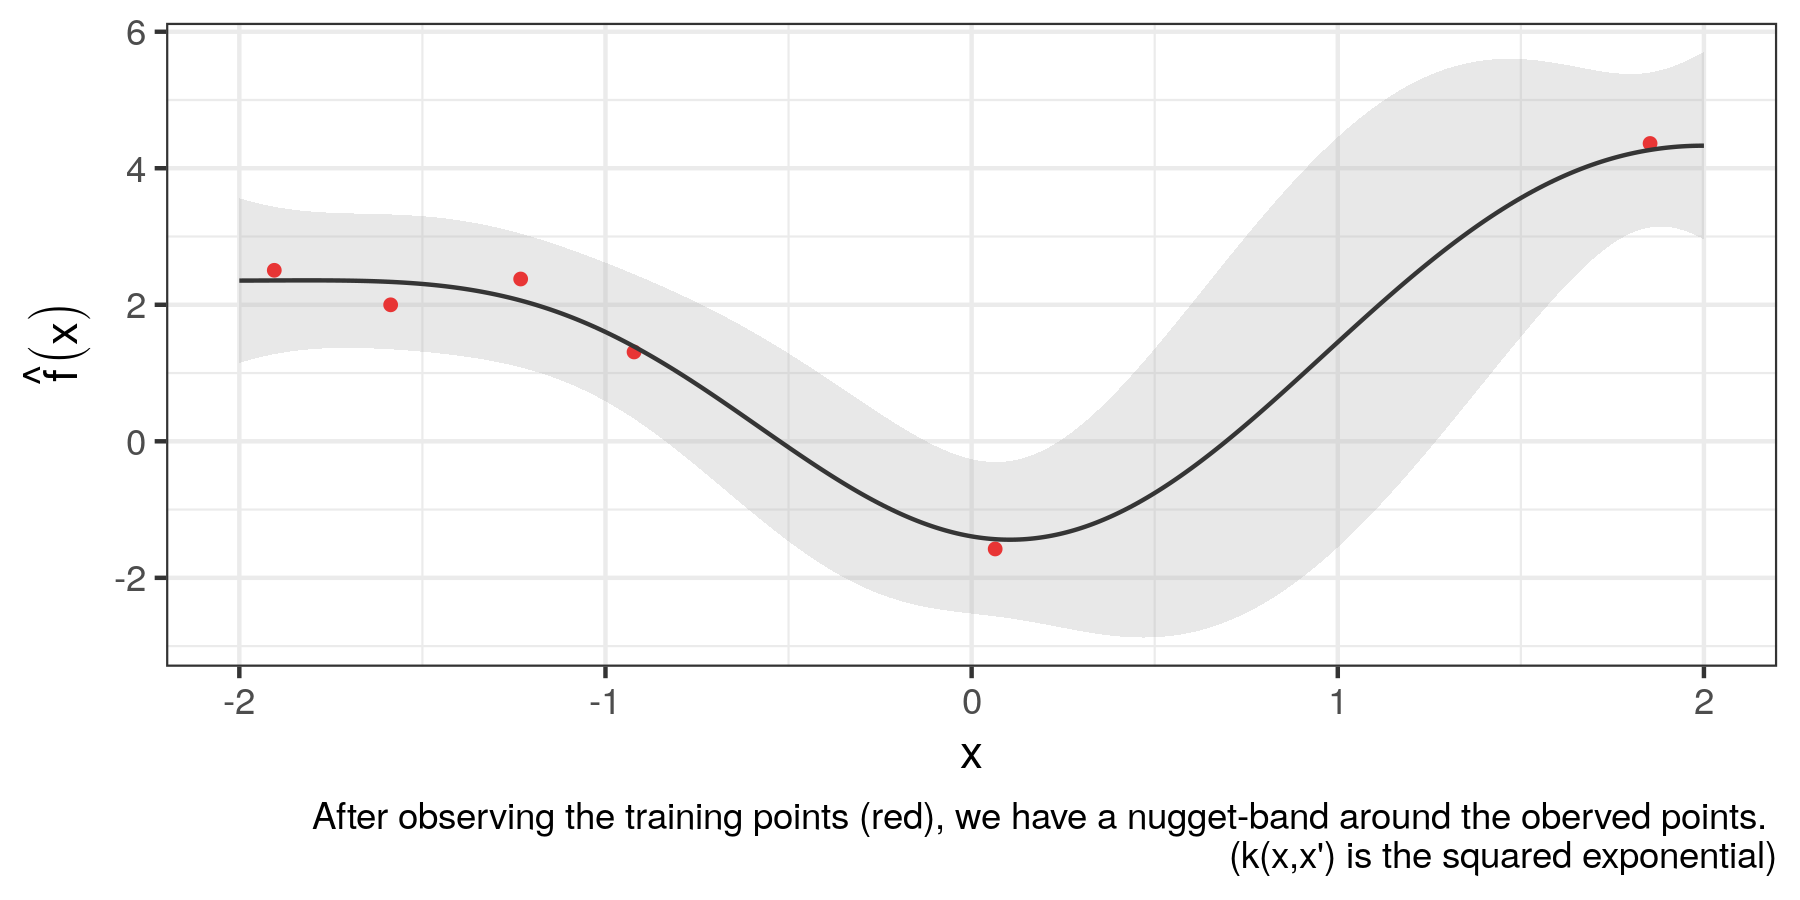
\includegraphics[width=0.6\textwidth]{figure_man/gp-regression.png}
\end{figure}

\end{frame}
%%%%%%%%%%%%%%%%%%%%%%%%%%%%%%%%%%%%%%%%%%%%%%%%%%%%%%%%%%%%%%%%%%%%%%%%%%%%%%%%%%%%
%\begin{frame}[c]{}
%\centering
%\huge
%\textbf{Decision Theory for Gaussian Processes}
%\end{frame}
%%%%%%%%%%%%%%%%%%%%%%%%%%%%%%%%%%%%%%%%%%%%%%%%%%%%%%%%%%%%%%%%%%%%%%%%%%%%%%%%%%%%%
%\begin{frame}[c,allowframebreaks]{Risk Minimization for Gaussian Processes}

%In machine learning, we usually choose a loss function and try to minimize the empirical risk:
%$$\riske(f) := \sum_{i=1}^{n}\loss(\yI{i},f(\xI{i})),$$

%as an approximation to the theoretical risk:
%$$\risk(f):= \expectation_{xy}[\loss(\y,f(\x))]= \int \loss(\y,f(\x)) \mathrm{d} \mathbb{P}_{x y}.$$

%\lz

%\begin{itemize}
%  \item How does the theory of Gaussian processes fit into this scenario? 
%  \lz
%  \item What if we were looking for predictions that atr optimal w.r.t. a certain loss function?
%\end{itemize}



%%%%%%%%%%%%%%%%%%%%%%%%%%%%%%%%%%%%%%%%%%%%%%%%%%%%%%%%%%%%%%%%%%%%%%%%%%%%%%%%%%%%%
%\framebreak


%\begin{itemize}

%\item The theory of Gaussian process provides us with a posterior distribution, i.e, $p(y ~|~\dataset).$

%\lz
  
%\item To make a prediction at a test point $\bm{x}_*$, we can approximate the theoretical risk by explointing the posterior distribution:
%$$\mathcal{R}(y_* ~|~ \bm{x}_*) \approx \int L(\tilde y_*, y_*) \, p(\tilde y_*~|~\bm{x}_*, \dataset)d\tilde y_*.$$
 
%\lz

%\item The optimal prediciton w.r.t the loss function is then: 
%$$\hat y_* ~|~ \bm{x}_* = \argmin_{y_*} \mathcal{R}(y_*~|~ \bm{x}_*)$$

%\end{itemize}


% \end{frame}

%%%%%%%%%%%%%%%%%%%%%%%%%%%%%%%%%%%%%%%%%%%%%%%%%%%%%%%%%%%%%%%%%%%%%%%%%%%%%%%%%%%%
\end{document}
